
\begingroup
\frametitle{ Ziel der Similarity Analysis}
% Similarity Analysis
\begin{frame}
	
	\begin{minipage}[t]{0.48\linewidth}
		\vspace*{-0.5em}
  \begin{itemize}
	\item Functional Similarity:
	\begin{itemize}
		\item Vergleich der Modellverhalten bei gleichen Aufgaben
		\item Sind die Ausgaben \( f(x) \) und \( f'(x) \) ähnlich?
	\end{itemize}
	\vspace{1em}
	\item Representational Similarity:
	\begin{itemize}
		\item Vergleich der internen Repräsentationen (z.B. Hidden States)
		\item Wie ähnlich sind die Zwischenrepräsentationen der Layer?
	\end{itemize}
\end{itemize}
	\end{minipage}
	\hfill
	\begin{minipage}[t]{0.49\linewidth}
		\vspace*{-0.5em}
		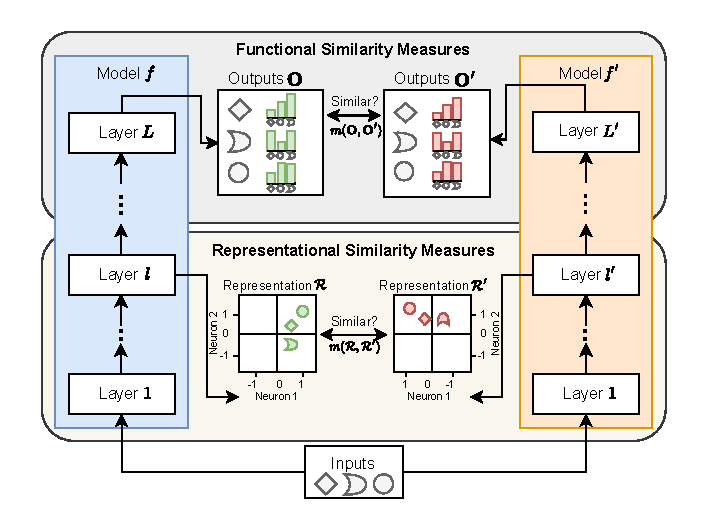
\includegraphics[width=1.2\linewidth]{BilderPräsentation/Similarity90Deg.drawio.pdf}
	\end{minipage}
	
\end{frame}
\endgroup


\begingroup
\frametitle{Vergleich durch internen Repräsentationen}
% Similarity Analysis
\begin{frame}

\uncover<1->{\begin{itemize}
	\item Repräsentation eines Modells $f$ auf Layer $l$
	\[
	R := R^{(l)} = (f^{(l)} \circ \dots \circ f^{(1)})(X) \in \mathbb{R}^{N \times D}
	\]
	\item $N$: Anzahl der Eingaben, $D$: Anzahl der Neuronen im Layer
	\item Repräsentationen \( R \) und \( R' \) können semantisch äquivalent sein, auch wenn sie sich numerisch unterscheiden.
	
\end{itemize}}

\vspace{-0.1em}
\uncover<2->{\begin{block}{Representational Similarity Measure}
		Eine Abbildung \( m(R, R') \) bewertet, wie ähnlich zwei Repräsentationen \( R, R' \in \mathbb{R}^{N \times D} \) sind.\\[0.2em]
		
\end{block}}

\vfill
{\tiny Quelle: Klabunde et al., “Similarity of Neural Network Models: A Survey of Functional and Representational Measures”, ACM Comput. Surv. 2020~\cite{klabunde_similarity_2024}}
\end{frame}
\endgroup

%\begingroup
%\frametitle{Vergleich durch internen Repräsentationen}
% Similarity Analysis
%\begin{frame}
%	\vspace{0.8em}
%\begin{block}{Invarianz eines Maßes}
%	Eine Abbildung $m$ ist \textbf{invariant} gegenüber $\mathcal{T}$, wenn \[
%	m(R, R') = m(\varphi(R), \varphi'(R')) \quad \forall \varphi, \varphi' \in \mathcal{T}\]
%\end{block}

%\vspace{0.8em}
%\begin{itemize}
%	\item Zwei Repräsentationen gelten als \textbf{$\mathcal{T}$-äquivalent}, wenn $\exists \psi \in \mathcal{T}$ mit $\psi(R) = R'$.
%	\item Schwächung des Metrik-Axioms:

%	\[
%	m(R, R') = 0 \iff R \sim_\mathcal{T} R'
%	\]
	%\textit{(Identität nur bis auf Transformationen)}
 %\end{itemize}
%\end{frame}
%\endgroup

